\chapter{GESTÃO DO PROJETO}
Nesta seção, serão apresentados os métodos escolhidos para a gestão do projeto e da equipe, com o objetivo de assegurar a melhor utilização possível do tempo, orçamento e recursos voltados para o projeto, para que esse possa ser concluído dentro do prazo estabelecido. Também serão levantados alguns riscos possíveis, afim de que com o conhecimento dessas possibilidades, medidas possam ser tomadas para evitá-los.  

\section{Formação da equipe}
A equipe foi formalizada durante as aulas da disciplina, porém já havia sido definida posteriormente. Todos os integrantes são alunos do curso de Tecnologia em Análise e Desenvolvimento de Sistemas, do Instituto Federal de São Paulo (IFSP), campus São Paulo. A equipe se baseia nos conhecimentos de cada um de seus membros com o objetivo de preencher as necessidades do projeto. Os participantes da equipe Noz são: 

\begin{itemize}
    \item \textbf{Kevin Klein}
    \item \textbf{Leonardo Tumani Teixeira Meireles}
    \item \textbf{Luiz Fernando Cavalcante de Faria}
    \item \textbf{Pedro Felipe da Silva Dias}
    \item \textbf{Ruan de Souza Cardoso Brito}
\end{itemize}

\subsection{Papéis}
Os papéis foram definidos através das habilidades dos membros , para que cada um pudesse atuar de maneira segura com seus conhecimentos, dessa maneira a organização e a fluidez do projeto são beneficiadas. As atividades são planejadas para que todos sejam responsáveis por alguma parte específica do projeto, podendo receber ajuda dos outros participantes caso seja necessário.

\newpage
\subsection{Organização da atividades}
    \item \begin{figure}[!htb]
 	    \centering
 	    \caption{\label{logo}Atividades de desenvolvimento}
 	    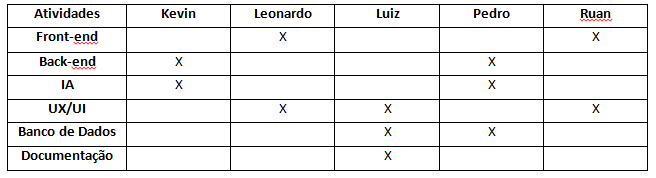
\includegraphics[width=16cm]{img/tabela-papeis-1.png}
\end{figure}


    \item \begin{figure}[!htb]
 	    \centering
 	    \caption{\label{logo}Atividades de gestão e planejamento}
 	    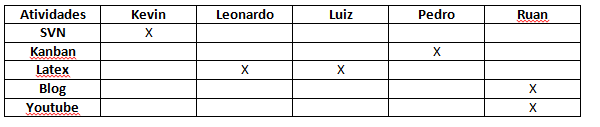
\includegraphics[width=16cm]{img/tabela-papeis-2.png}
\end{figure}

\section{Gestão de tempo e desenvolvimento}
A equipe decidiu aderir à utilização do Scrum como framework de gerenciamento, a fim de melhorar a organização durante o desenvolvimento do projeto. Ele foi escolhido pela sua eficiência e ampla utilização por diversas empresas no mercado, além de ser conhecido pelos integrantes do grupo, o que facilita sua implementação.  Além disso também optamos pela utilização do Kanban, para garantir a eficiência na realização das tarefas e o cumprimento dos prazos.

\subsection{Scrum}
O Scrum é uma metodologia de desenvolvimento ágil amplamente empregada para lidar com a complexidade na criação de produtos. Este método valoriza a colaboração, a autonomia da equipe e a entrega progressiva e iterativa. Composto por uma série de práticas, papéis e artefatos, o Scrum promove a eficácia e a qualidade do trabalho realizado, impulsionando a entrega de valor de forma consistente ao longo do tempo.

\subsection{Kanban}
O Kanban é uma metodologia de gestão visual que teve origem no Japão e ganhou popularidade em diversos setores, como desenvolvimento de software, manufatura e serviços. O termo "Kanban" significa "sinal visual" em japonês, e essa abordagem se baseia na utilização de cartões ou post-its para representar unidades de trabalho e visualizar o fluxo do processo. Essa metodologia visa proporcionar transparência sobre o trabalho em andamento e controlar o trabalho em progresso (WIP) para otimizar a eficiência do sistema.

\section{Gestão de comunicação}
A comunicação é parte essencial para que tudo corra bem no projeto. Foram utilizados alguns meios para realizar esse diálogo entre a equipe.

O meios de comunicação utilizados internamente foram o  Whatsapp, aplicativo de mensagens instantâneas  e chamadas de voz, foi usado para troca de mensagens durantes as semanas, a fim de proporcionar agilidade e facilidade na comunicação, e o Discord, que é uma aplicação voltada para a comunicação, principalmente de grupos e comunidades, foi usado para as reuniões realizadas semanalmente.

Para a comunicação com o público foram criados um blog, na plataforma Blogger, onde são compartilhadas as atualizações semanais e informações relevantes sobre o projeto.

 \begin{figure}[!htb]
 	    \centering
 	    \caption{\label{logo}QRCode do Blog}
 	    
\includegraphics[width=5cm]{img/qrcode-blog.png}
 	    \fonte{Os autores.}
\end{figure}
\FloatBarrier

 \begin{figure}[!htb]
 	    \centering
 	    \caption{\label{logo}QRCode do Youtube}
 	    
\includegraphics[width=5cm]{img/qrcode-youtube.png}
 	    \fonte{Os autores.}
\end{figure}
\FloatBarrier

\section{Análise de riscos}
Nessa seção é possível avaliar alguns dos possíveis riscos ao projeto, analisando seu nível de impacto e qual o tipo de resposta para cada um em específico.

\begin{figure}[!htb]
 	    \centering
 	    \caption{\label{logo}Análise de riscos}
 	    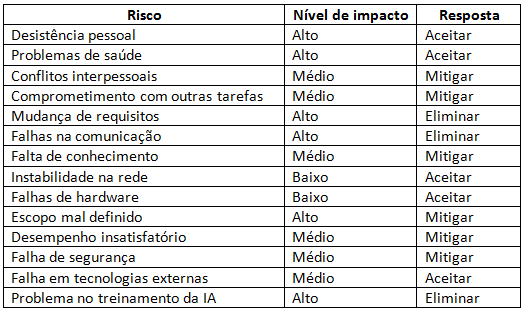
\includegraphics[width=15cm]{img/riscos.png}
\end{figure}

Segue abaixo uma breve explicação sobre cada um dos possíveis riscos ao projeto:

\begin{itemize}
    \item \textbf{Desistência pessoal:} Membros da equipe abandonam o projeto, causando lacunas na expertise e sobrecarregando os membros restantes.
    \item \textbf{Problemas de saúde:} Membros da equipe enfrentam problemas de saúde que afetam sua capacidade de contribuir para o projeto.
    \item \textbf{Conflitos interpessoais:} Desentendimentos ou tensões entre membros da equipe prejudicam a colaboração e a eficiência do projeto.
    \item \textbf{Comprometimento com outras tarefas:} Membros da equipe têm prioridades divididas entre várias tarefas ou projetos, resultando em atrasos ou falta de dedicação ao projeto em questão.
    \item \textbf{Mudança de requisitos:} Alterações nos requisitos do projeto após o início do desenvolvimento, levando a retrabalho e atrasos.
    \item \textbf{Falhas na comunicação:} Comunicação inadequada entre membros da equipe, clientes ou partes interessadas, levando a mal-entendidos e erros.
    \item \textbf{Falta de conhecimento:} Membros da equipe não possuem as habilidades ou conhecimentos necessários para concluir com sucesso determinadas tarefas ou aspectos do projeto.
    \item \textbf{Instabilidade na rede:} Problemas com a conexão de rede afetam a colaboração remota ou o acesso a recursos necessários para o projeto.
    \item \textbf{Falhas de hardware:} Hardware essencial para o projeto falha, causando interrupções no desenvolvimento ou perda de dados.
    \item \textbf{Escopo mal definido:} Requisitos do projeto não estão claramente definidos desde o início, levando a confusão e revisões frequentes.
    \item \textbf{Desempenho insatisfatório:} O produto final não atende às expectativas de desempenho dos usuários, levando à insatisfação e possível rejeição.
    \item \textbf{Falha de segurança:} Vulnerabilidades de segurança no sistema comprometem a integridade ou a confidencialidade dos dados, resultando em riscos para os usuários e para a empresa.
    \item \textbf{Falha em tecnologias externas:} Dependência de tecnologias externas que podem falhar ou não atender às expectativas, afetando o desenvolvimento ou o funcionamento da aplicação.
    \item \textbf{Problema no treinamento da IA:} Dificuldades no treinamento de sistemas de inteligência artificial para alcançar os resultados desejados, resultando em desempenho inadequado ou inexato.
\end{itemize}